\documentclass{article}
\usepackage[ascii]{inputenc}
\usepackage[T1]{fontenc}
\usepackage[english]{babel}
\usepackage{amsmath}
\usepackage{amssymb,amsfonts,textcomp}
\usepackage{color}
\usepackage{array}
\usepackage{supertabular}
\usepackage{hhline}
\usepackage[normalem]{ulem}
\usepackage{hyperref}
\usepackage{textcomp}
\usepackage{layout}
\usepackage[numbers]{natbib}
\usepackage{caption}
\usepackage{booktabs}       % professional-quality tables

\hypersetup{colorlinks=true, linkcolor=black, citecolor=black, filecolor=blue, urlcolor=blue, pdftitle=CAD17abstract, pdfauthor=Orest Mykhaskiv, pdfsubject=, pdfkeywords=}
\usepackage[pdftex]{graphicx}

\newcommand\textstyleInternetlink[1]{\textcolor{blue}{#1}}

\setcounter{secnumdepth}{2}
\renewcommand\thesection{\arabic{section}}
\renewcommand\thesubsection{\arabic{section}.\arabic{subsection}}
\makeatletter
\newcommand\arraybslash{\let\\\@arraycr}
\makeatother

\newcommand\liststyleWWviiiNumxxxiii{%
\renewcommand\labelitemi{{\textbullet}}
\renewcommand\labelitemii{{}-}
\renewcommand\labelitemiii{${\blacksquare}$}
\renewcommand\labelitemiv{{\textbullet}}
}
\newcommand\liststyleWWviiiNumxxix{%
\renewcommand\labelitemi{{\textbullet}}
\renewcommand\labelitemii{o}
\renewcommand\labelitemiii{${\blacksquare}$}
\renewcommand\labelitemiv{{\textbullet}}
}
\newcommand\liststyleWWviiiNumxxiv{%
\renewcommand\labelitemi{{\textbullet}}
\renewcommand\labelitemii{o}
\renewcommand\labelitemiii{${\blacksquare}$}
\renewcommand\labelitemiv{{\textbullet}}
}
\newcommand\liststyleWWviiiNumxxi{%
\renewcommand\labelitemi{{\textbullet}}
\renewcommand\labelitemii{o}
\renewcommand\labelitemiii{${\blacksquare}$}
\renewcommand\labelitemiv{{\textbullet}}
}
\newcommand\liststyleWWviiiNumxxiii{%
\renewcommand\labelitemi{{\textbullet}}
\renewcommand\labelitemii{o}
\renewcommand\labelitemiii{${\blacksquare}$}
\renewcommand\labelitemiv{{\textbullet}}
}
\newcommand\liststyleWWviiiNumxv{%
\renewcommand\labelitemi{{\textbullet}}
\renewcommand\labelitemii{o}
\renewcommand\labelitemiii{${\blacksquare}$}
\renewcommand\labelitemiv{{\textbullet}}
}
\newcommand\liststyleWWviiiNumxxx{%
\renewcommand\theenumi{\arabic{enumi}}
\renewcommand\theenumii{\alph{enumii}}
\renewcommand\theenumiii{\roman{enumiii}}
\renewcommand\theenumiv{\arabic{enumiv}}
\renewcommand\labelenumi{[\theenumi]}
\renewcommand\labelenumii{\theenumii.}
\renewcommand\labelenumiii{\theenumiii.}
\renewcommand\labelenumiv{\theenumiv.}
}
\newcommand\liststyleWWviiiNumxxxii{%
\renewcommand\labelitemi{{\textbullet}}
\renewcommand\labelitemii{o}
\renewcommand\labelitemiii{${\blacksquare}$}
\renewcommand\labelitemiv{{\textbullet}}
}

\renewcommand\refname{}
\renewcommand{\bibsection}{}
\renewcommand{\theequation}{2.\arabic{equation}}


\setlength\paperwidth{19.05cm}
\setlength\paperheight{26.162cm}
\setlength\voffset{-1in}
\setlength\hoffset{-1in}
\setlength\topmargin{30pt}
\setlength\oddsidemargin{1.524cm}
\setlength\textheight{576pt}
\setlength\textwidth{16.001999cm}
\setlength\footskip{0.841cm}
\setlength\headheight{16pt}
\setlength\headsep{28pt}


\usepackage{fancyhdr}
\pagestyle{fancy}
\fancyhf{}
\renewcommand{\headrulewidth}{0pt}
\renewcommand{\footrulewidth}{0.4pt}
\fancyhead[R]{\thepage}
\fancyfoot[R]{Proceedings of CAD'21, Barcelona, Spain, July 5-7, 2021, aaa-bbb\\ {\footnotesize{\textcopyright}} 2021 CAD Solutions, LLC, \ULurl{http://www.cad-conference.net}}

\usepackage{etoolbox}
\patchcmd{\thebibliography}{\section*{\refname}}{}{}{}
\captionsetup[figure]{labelformat={default},name={Fig.}}

\setlength{\bibsep}{2pt plus 0.3ex}
\setcounter{page}{1}

\makeatletter
\DeclareUrlCommand\ULurl@@{%
  \def\UrlFont{\ttfamily\color{blue}}%
  \def\UrlLeft{\uline\bgroup}%
  \def\UrlRight{\egroup}}
\def\ULurl@#1{\hyper@linkurl{\ULurl@@{#1}}{#1}}
\DeclareRobustCommand*\ULurl{\hyper@normalise\ULurl@}
\makeatother

\begin{document}

{\centering  
\includegraphics[width=5.173cm,height=2.193cm]{images/CADconverted-img001.jpg} \par}

\vspace{5pt}
\noindent
\underline{Title:}

\noindent{\bfseries
MidcurveNN: Neural Network for Computing Midcurve of a Thin Polygon }

\vspace{1em}
\noindent \underline{Authors:}
\newline
Yogesh Kulkarni, yogeshkulkarni@yahoo.com, Pune, India.

\vspace{1em}
\noindent \underline{Keywords:}\newline
Midcurve, Medial-axis Transform, Encoder-Decoder, Neural Networks


\bigskip


\noindent \underline{DOI:} 10.14733/cadconfP.2021.xxx-yyy

\vspace{10pt}
\noindent\underline{Introduction:}\vspace{0.2em}\newline
A skeleton is a lower dimensional entity which represents shape of its parent object. It being simpler than the parent object, operations like pattern recognition, approximation, similarity estimation, collision detection, animation, matching and deformation can be performed efficiently on it than on the parent object. 

Skeletons, also known as Medial Objects, can be computed via various mathematical formulations/approaches such as Medial Axis Transform (MAT), Chordal Axis Transform (CAT), Pairing, Thinning etc. Figure \ref{fig_medialmethods} shows some of these. More detailed analysis can be found in the survey paper \cite{medial2010}.

    \begin{center}
	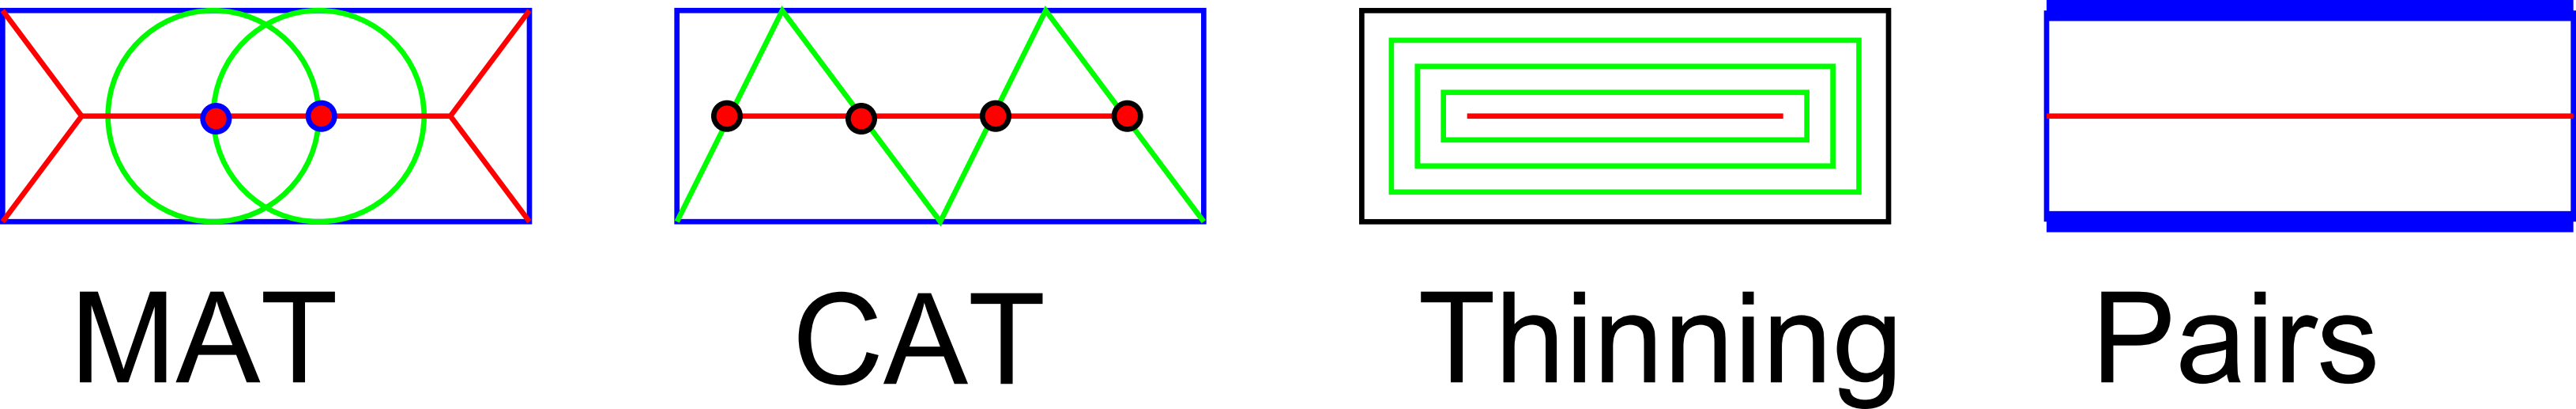
\includegraphics[width=0.6\linewidth]{images/MedialMethodsOnlyShort}
	\captionof{figure}{Medial Object computation methods}
	\label{fig_medialmethods}
    \end{center}
    

In the current paper we focus on computing midcurve for 2D planar sketch profiles.  Even in 2D profiles, shapes vary enormously. As the first level of simplification, we would deal with 2D polygons only (with an assumption that curved shapes can be converted to polygonal shape by faceting). Figure \ref{fig_letters} shows some of the input shapes which can be considered. English alphabets are chosen for easy understanding and verification of the proposed method.

     \begin{center}
	
\includegraphics[width=0.6\linewidth]{images/Letters}
	\captionof{figure}{2D Thin Polygonal shapes}
	\label{fig_letters}
    \end{center}


\vspace{10pt}
\noindent\underline{Proposed Method:}\vspace{0.2em}\newline
Computation of midcurve, in its original form, is transformation of a 2D thin closed, with/without-holes polygon to 1D open/closed/branched polyline. Paper \cite{dimred2017} details one of the effective midcurve computation techniques, based on rule-based computational geometry approach. Such techniques have a shortcoming of not being scalable or generic enough to be able to handle variety of shapes. Deep Learning neural network architectures are showing potential of developing such generic models. This dimension reduction transformation should ideally be modeled as Sequence to Sequence (Seq2Seq) neural architecture, like Machine Translation. In the current problem, the input and the output sizes could be different not just in a single sample, but across all samples. Many current Seq2Seq neural networks need fixed size inputs and outputs, which if not present in data, are artificially managed by adding padding of certain improbable value. Such padding is not appropriate for the current midcurve computation problem, as the padding-value can inappropriately get treated as part of the valid input. In this initial phase, to circumvent the problem of variable size, image-based inputs and outputs are used, which are of fixed size. Both input and output polygonal shapes are rasterized into images of 100x100, thus making them fixed size for all samples, irrespective of the original shapes.

This paper proposes to use such network for midcurve computation in the form of image-to-image mode. Input images have thin polygonal shapes whereas output images have corresponding midcurve images. Figure \ref{fig_endecoder} shows the Encoder-decoder architecture, called MidcurveNN.

     \begin{center}
	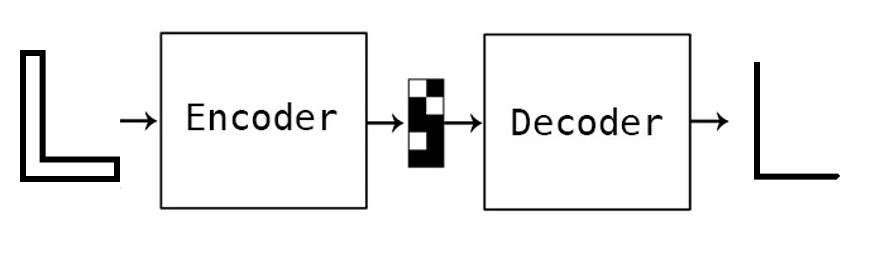
\includegraphics[width=0.6\linewidth]{images/midcurve_encoder_decoder}
	\captionof{figure}{Encoder-Decoder Architecture}
	\label{fig_endecoder}
    \end{center}
    
Input and output geometries are rasterized into 100x100 size images. Transformations like translation, rotation and mirroring are applied to create diversity in the samples. MidcurveNN being a Supervised Learning approach, both input thin-polygons and corresponding output midcurve polylines are transformed simultaneously. Figure \ref{fig_training} shows some samples. This is training data.    


     \begin{center}
	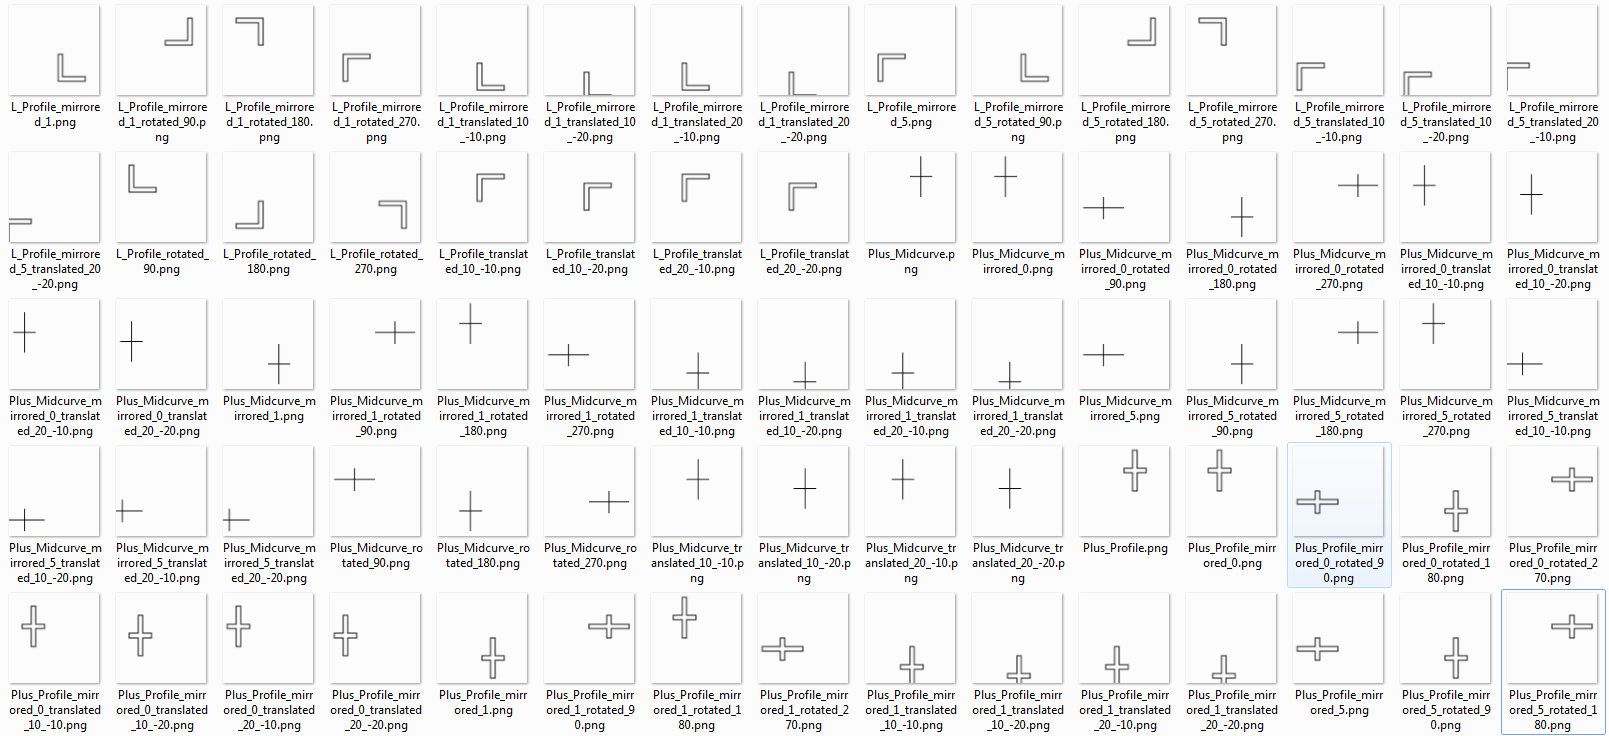
\includegraphics[width=\linewidth]{images/training_data}
	\captionof{figure}{Training Data: Inputs (thin polygons) and outputs (midcurves)}
	\label{fig_training}
    \end{center}
    
MidcurveNN encoder-decoder has been implemented in Python programming with Keras library \cite{autoenkeras}.  Encoder takes input image of size $100 \times 100 = 10000$, then comes Dense layer with size $100$ to form the encoded vector. Decoder takes encoded vector as input, then with a Dense layer expands back to $100 \times 100 = 10000$ size of the output image. Relu activation is used for Encoder whereas Sigmoid for the decoder. AdaDelta optimizer with binary cross entropy as loss function is used to compute the losses. Table \ref{tbl_loss} shows loss across number of epochs.    


\begin{table}
\captionof{table}{Improvement in performance with epochs}
\centering

\begin{tabular}[htbp]{@{} p{0.14\linewidth}  p{0.22\linewidth}  p{0.22\linewidth}  @{}} \toprule
{\bf Epochs } & {\bf Training loss }  & {\bf Validation loss} \\
\midrule
50	& -17.6354	& -8.3223\\
200	& -16.8878	& -7.7672 \\
\bottomrule
\end{tabular}
\label{tbl_loss}
\end{table}


Some of the results are shown in Figure \ref{fig_results}. Inputs are at the top and output midcurve at the bottom.

     \begin{center}
	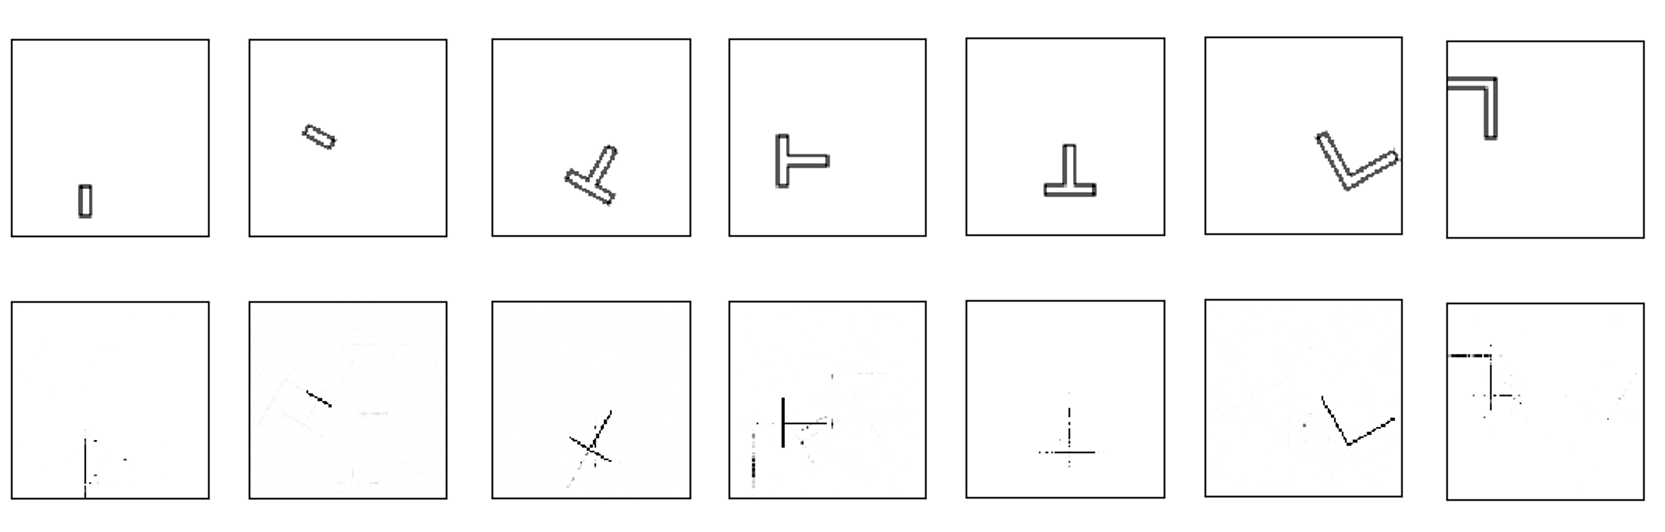
\includegraphics[width=\linewidth]{images/midcurvenn_results}
	\captionof{figure}{Predicted Data: Inputs (thin polygons) and outputs (midcurves)}
	\label{fig_results}
    \end{center}

Shape on the top is the input thin polygon whereas the corresponding shape at the bottom is the predicted midcurve. It can be clearly seen that the network is able to localize the shape and learn the dimension reduction function reasonably well. It is still not perfect or usable, as some stray points are still being wrongly classified as the part of output midcurve. A better network model and/or post processing is needed to make output midcurve practically usable.


\vspace{1em}
\noindent\underline{Conclusions and Future Work:}\vspace{0.2em}\newline
Traditional methods of computing midcurves are predominantly rules-based and thus, have limitation of not developing a generic model which will accept any input shape. MidcurveNN, a novel Encoder-Decoder network attempts to build such a generic model. This paper demonstrates that simple single layer encoder and decoder network can learn the dimension reduction function reasonably well. Although more development is necessary in evolving a better neural architecture, the current results show positive potential. 

Working on truly variable size inputs (thin polygon) and outputs (polyline) using dynamic graph of Encoder-Decoder network can be attempted in the future. More and highly diversified data can help improve the quality of the output. Developing a formal representation of polygonal shapes with variations such as open/closed, with-without loops, branched as a coherent sequence of points is also on the agenda.

% \vspace{1em}
% \noindent\underline{Acknowledgement:}\vspace{0.2em}\newline
% This research is a part of the IODA project - Industrial Optimal Design using Adjoint CFD. IODA is \textit{Marie Sklodowska-Curie Innovative Training Network} funded by European Commission under Grant Agreement No.~642959.

% \vspace{1em}
% \noindent\underline{IMPORTANT NOTES:}\vspace{0.2em}\newline
% WE ARE REQUIRED BY CROSSREF TO INCLUDE HYPERLINK INTO EVERY REFERENCE THAT HAS DOI LINKING. PLEASE GO TO: \ULurl{http://www.crossref.org/SimpleTextQuery/}, REGISTER YOUR E-MAIL, CUT AND PASTE THE LIST OF REFERENCES INTO THE BOX, GET THE DOI LINKS AND PASTE THEM INTO YOUR PAPER! THE LINKS SHOULD LOOK LIKE THIS, I.E. USE HTTPS AND DROP THE DX: \ULurl{https://doi.org/10.1080/16864360.2014.881190}


\vspace{1em}
\noindent\underline{References:}\vspace{-1.9em}\newline
\renewcommand{\section}[2]{}
\begin{thebibliography}{9}

\bibitem{autoenkeras}
Chollet, F.
\newblock Building Autoencoders in Keras
\newblock In {\em https://blog.keras.io/building-autoencoders-in-keras.html }, 2019.


\bibitem{medial2010}
Kulkarni, Y. H.; Deshpande, S.
\newblock Medial Object Extraction - A State of the Art
\newblock In {\em International Conference on Advances in Mechanical Engineering, SVNIT, Surat}, 2010.  

\bibitem{dimred2017}
Kulkarni, Y. H.; Sahasrabudhe, A.D.; Kale, M.S
\newblock Dimension-reduction technique for polygons
\newblock In {\em International Journal of Computer Aided Engineering and Technology, Vol. 9, No. 1}, 2017. \ULurl{https://doi.org/10.1504/IJCAET.2017.080772}
\end{thebibliography}



\end{document}
